

\section{Distribución de Poisson}

Supongamos que estamos interesados en conteos que ocurren en un intervalo de
tiempo (por ejemplo, dentro de una hora en particular). Debido a que son
conteos, no son negativos y tienen un valor entero. Sabemos que estos recuentos
tienen dos propiedades importantes. Primero, ocurren con alguna tasa promedio
fija. En segundo lugar, se produce una observación independientemente del
intervalo desde la última observación. Entonces la distribución de Poisson es un
modelo apropiado \cite{forsyth2018probability}.

\begin{theorem}{Distribución de Poisson}{Poisson}
Una variable aleatoria $X$, no negativa de valor entero, tiene una distribución de
Poisson cuando su distribución de probabilidad toma la forma:

\begin{equation}
    P({X=k})=\lambda^k e^{-\lambda}
\end{equation}

Donde $\lambda > 0$ es un parámetro conocido como la intensidad de la distribución.
    
\end{theorem}

La distribución de Poisson es una distribución de probabilidad, porque es no
negativa y porque:

\begin{center}
    \[
\sum_{i=0}^{\infty} \frac{\lambda^i}{i!} = e^\lambda
\]
\end{center}

tal que,

\begin{center}
    \[
\sum_{k=0}^{\infty} \frac{\lambda^i e^\lambda}{i!}  = 1
\]
\end{center}

Una distribución de Poisson con intensidad $\lambda$ tiene:

\begin{itemize}
    \item Media $\lambda$;
    \item Varianza $\lambda$
\end{itemize}

La distribución de Poisson se usa a menudo en situaciones en las que contamos el
número de éxitos en una región o intervalo de tiempo en particular, y hay una
gran cantidad de intentos, cada uno con una pequeña probabilidad de éxito
\cite{blitzstein2015introduction}.

Por ejemplo, las siguientes variables aleatorias podrían seguir una distribución
que es aproximadamente Poisson.

\begin{itemize}
\item El número de correos electrónicos que recibe en una hora. Hay muchas
personas que potencialmente podrían enviar un correo electrónico en esa hora,
pero es poco probable que una persona específica realmente le envíe un correo
electrónico en esa hora. Alternativamente, imagina subdividir la hora en
milisegundos. Hay $3.6 \times 10^6$ segundos en una hora, pero en cualquier
milisegundo específico es poco probable que reciba un correo electrónico.

\item El número de chispas en una galleta con chispas de chocolate. Imagina
subdividir la galleta en cubos pequeños; la probabilidad de obtener una chispa
de chocolate en un solo cubo es pequeña, pero el número de cubos es grande.

\item El número de terremotos en un año en alguna región del mundo. En cualquier
momento y lugar dados, la probabilidad de un terremoto es pequeña, pero hay una
gran cantidad de posibles momentos y lugares para que ocurran terremotos en el
transcurso del año.

\end{itemize}

\subsection{Aproximación a la distribución de Poisson a partir de la Binomial.}

La distribución binomial depende de 3 parámetros:

  \begin{equation}
    f(x,n,p) = \binom{n}{x} p^x (1-p)^{n-x}
  \end{equation}

Entonces, queremos saber si existe una relación entre el experimento actual y el
anterior.

Por lo que podemos hacer:

\begin{equation}
  \begin{array}{rr}
  \frac{f(x,n,p)}{f(x-1,n,p)} = & \frac{\binom{n}{x} p^x (1-p)^{n-x}}{\binom{n}{x-1} p^{x-1} (1-p)^{n-(x-1)}} \\
  \\
%                              = & \frac{\binom{n}{x} p^x (1-p)^{n} (1-p)^{-x}}{\binom{n}{x-1} \frac{p^x}{p} (1-p)^{n}(1-p)^{-(x-1)}} \\

                              = & \frac{\binom{n}{x} p^x (1-p)^{n} (1-p)^{-x}}{\binom{n}{x-1} \frac{p^x}{p} (1-p)^{n}(1-p)^{-x} (1-p)}
  \end{array}
\end{equation}

\begin{equation}
  \begin{array}{rr}
  \frac{f(x,n,p)}{f(x-1,n,p)} = & \frac{\binom{n}{x} p}{\binom{n}{x-1} (1-p)} \\
  \\
                              = & \frac{\binom{n}{x} p}{\binom{n}{x-1} q} \\
  \end{array}
\end{equation}

Pero...
  
\begin{equation}
  \begin{array}{rr}
  \frac{\binom{n}{x}}{\binom{n}{x-1}} = & \frac{\frac{n!}{(n-x)!x!}}{\frac{n!}{(n-(x-1))!(x-1)!}} \\
  \\
                                      = & \frac{n-x+1}{x}
  \end{array}
\end{equation}

Por lo que...

\begin{equation}
  \begin{array}{rr}
  \frac{f(x,n,p)}{f(x-1,n,p)} = & \frac{n-x+1}{x} \cdot \frac{p}{q}
  \end{array}
\end{equation}

\begin{equation}
  \begin{array}{rr}
  \frac{f(x,n,p)}{f(x-1,n,p)} = & \frac{(n+1)p - xp}{xq} \\
  \\
                              = & \frac{(n+1)p - x(1-q)}{xq} \\
  \\
                              = & \frac{(n+1)p - x + xq}{xq} \\
  \\
                              = & 1 + \frac{(n+1)p - x}{xq} \\
  \end{array}
  \label{eq:poissonGral}
\end{equation}

Ahora podemos hacer el caso cuando $x=0$:

\begin{equation}
  f(0,n,p) = \binom{n}{0} p^0 (1-p)^{n-0} = (\frac{n!}{(n-0)! 0!})(1-p)^n = (1-p)^n
\end{equation}

Pero sabemos que la esperanza matemática $\lambda = np \Rightarrow p =
\frac{\lambda}{n}$,
  
entonces,

\begin{equation}
  f(0,n,p) = (1-\frac{\lambda}{n})^n
\end{equation}

Podemos hacer que:

\begin{equation}
  \ln(f(0,n,p)) = n \ln((1-\frac{\lambda}{n}))
\end{equation}

Usando la serie de Taylor:

\begin{equation}
  \ln(1+x) = x - \frac{x^2}{2} + \frac{x^3}{3} - \frac{x^4}{4} + ...
\end{equation}

Tenemos que:

\begin{equation}
  \begin{array}{rl}
  \ln(1+(-\frac{\lambda}{n})) = & (-\frac{\lambda}{n}) - \frac{(-\frac{\lambda}{n})^2}{2} + \frac{(-\frac{\lambda}{n})^3}{3} - \frac{(-\frac{\lambda}{n})^4}{4} + ... \\
  \\
                              = & -\frac{\lambda}{n} + \frac{\lambda^2}{2n^2} - \frac{\lambda^3}{3n^3} - \frac{\lambda^4}{4n^4}+...
  \end{array}
\end{equation}

Pero sabemos que $n \to \infty$, por lo que nos queda:

\begin{equation}
  n \ln(1-\frac{\lambda}{n}) = -\lambda
\end{equation}  

Sabiendo que: \\

$ \lim_{n \to \infty} [\ln (f(0,n,p))] = \lim_{n \to \infty} (1 -
\frac{\lambda}{n})^n = -\lambda$


Quitando el $\ln$, podemos concluir que para $n=0$,

\begin{equation}
  f(0,n,p) = e^{-\lambda}
\end{equation}

Si $x=1$, a partir de la Ec. \eqref{eq:poissonGral}, tenemos:

\begin{equation}
  \begin{array}{rl}
  f(1,n,p)  = & (1 + \frac{(n+1)p - 1}{q}) \cdot f(0,n,p) \\
  \\
            = & (\frac{q + (n+1)p - 1}{q}) \cdot e^{-\lambda} \\
  \\
            = & (\frac{q + p + np - 1}{q}) \cdot e^{-\lambda} \\
  \\
            = & (\frac{np}{q}) \cdot e^{-\lambda} \\
  \\
            = & (\frac{\lambda}{q}) \cdot e^{-\lambda} \\
  \end{array}
\end{equation}

Siempre que $n \to \infty$ y $p \to 0 \Rightarrow q \to 1$, porque $q=1-p$
Entonces:

\begin{equation}
f(1,n,p) = \lambda e^{-\lambda}
\end{equation}

Si $x=2$, a partir de la Ec. \eqref{eq:poissonGral}, tenemos:

\begin{equation}
  \begin{array}{rl}
  f(2,n,p)  = & (1 + \frac{(n+1)p - 2}{2q}) \cdot f(1,n,p) \\
  \\
            = & (\frac{2q + (n+1)p - 2}{2q}) \cdot \lambda e^{-\lambda} \\
  \\
            = & (\frac{2q + np + p - 2}{2q}) \cdot \lambda e^{-\lambda} \\
  \\
            = & (\frac{2(1-p) + np + p - 2}{2q}) \cdot \lambda e^{-\lambda} \\
  \\
            = & (\frac{2 - 2p + np + p - 2}{2q}) \cdot \lambda e^{-\lambda} \\
  \\
            = & (\frac{np - p}{2q}) \cdot \lambda e^{-\lambda} \\
  \end{array}
\end{equation}

Pero $np=\lambda$

\begin{equation}
  f(2,n,p)  = (\frac{\lambda - p}{2q}) \cdot \lambda e^{-\lambda}
\end{equation}

Pero si $p \to 0$, entonces $q \to 1$ porque $q=1-p$
Entonces, tenemos que:

\begin{equation}
  f(2,n,p)  = (\frac{\lambda}{2}) \cdot \lambda e^{-\lambda}
\end{equation}

Sabemos que si $x=0$: \\
$f(0,n,p) = \frac{\lambda^0}{0!} e^{-\lambda}$\\

Si $x=1$: \\
$f(1,n,p) = \frac{\lambda^1}{1!} e^{-\lambda}$\\

Si $x=2$: \\
$f(2,n,p)  = \frac{\lambda^2}{2!} \cdot \lambda e^{-\lambda}$\\


Entonces, si $x=k$:

\begin{equation}
  f(k,n,p)  = \frac{\lambda^k}{k!} \cdot \lambda e^{-\lambda}
\end{equation}

Esta es la función de probabilidad de Poisson de V.A. Así, podemos definir tres
parámetros importantes:

\begin{enumerate}
  \item Valor esperado:
  \begin{equation}
    \mu = E(x) = \sum_{x} xf(x) = \sum_{x} \frac{x e^{-\lambda}\lambda^k}{x!} = \lambda
  \end{equation}

\item Varianza:
\begin{equation}
  \sigma^2 = \sum_{x} \frac{x^2 e^{-\lambda}\lambda^k}{x!} - (\sum_{x} \frac{x e^{-\lambda}\lambda^k}{x!})^2 = \lambda
\end{equation}

\item Desviación estándar:
\begin{equation}
  \sigma = \sqrt{\lambda}
\end{equation}

\end{enumerate}

\subsection{Ejemplo de la distribución de Poisson}

El número de incidentes de tránsito que ocurren en una cierta avenida en un día
cualquiera sigue una distribución Poisson de media $\lambda=1$. Entonces:

  \begin{figure}
    \centering
    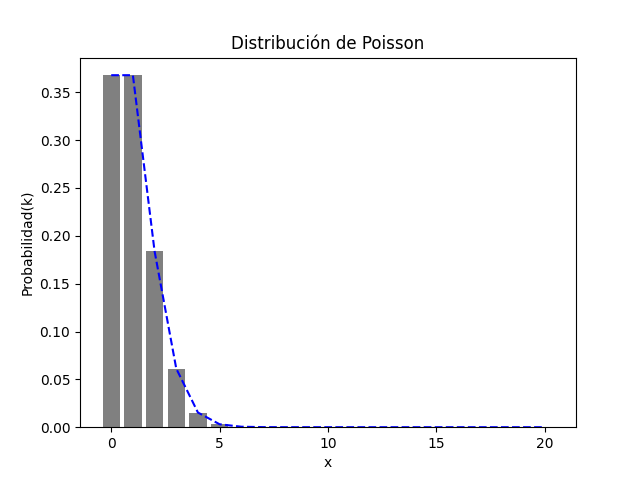
\includegraphics[scale=0.6]{../slides/figures/poisson_distribution_lambda_1.png}
  \end{figure}

El número de incidentes de tránsito que ocurren en una cierta avenida en un día
cualquiera sigue una distribución Poisson de media $\lambda=4$. Entonces:

  \begin{figure}
    \centering
    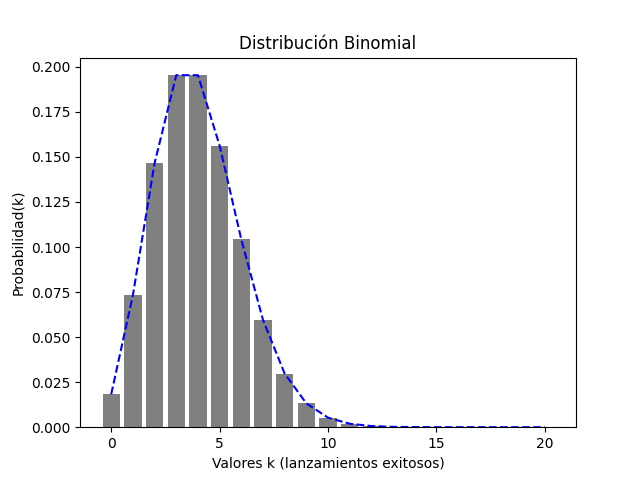
\includegraphics[scale=0.6]{../slides/figures/poisson_distribution_lambda_4.png}
  \end{figure}

El número de incidentes de tránsito que ocurren en una cierta avenida en un día
cualquiera sigue una distribución Poisson de media $\lambda=10$. Entonces:

\begin{figure}
    \centering
  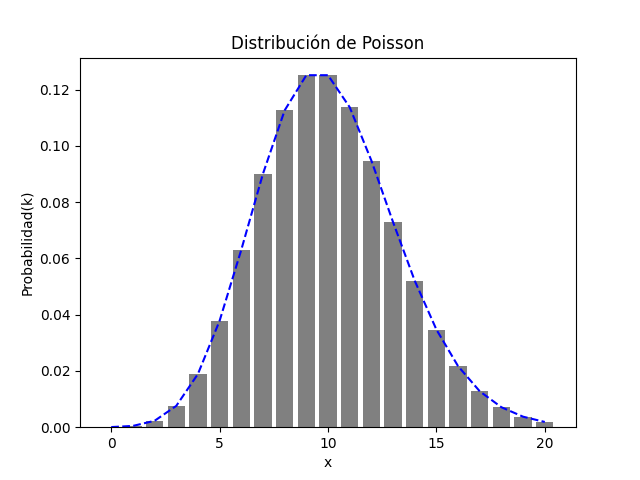
\includegraphics[scale=0.6]{../slides/figures/poisson_distribution_lambda_10.png}
\end{figure}

